\documentclass[12pt, a4paper, twocolumn]{article}
\usepackage[utf8]{inputenc}
\usepackage{graphicx}
\usepackage{amsmath}
\usepackage{booktabs}
\usepackage{hyperref}
\usepackage{geometry}
\usepackage{float}
\geometry{margin=1in}

\title{Synthetic Data Generation Using GANs}
\author{Mukunda Reddy}
\date{}

\begin{document}

\maketitle

\section{Introduction}
Synthetic data refers to artificially generated data that mimics the properties of real-world datasets. It is widely used to augment training sets, preserve privacy, and overcome challenges such as data scarcity or imbalance. In recent years, generative adversarial networks (GANs) have emerged as a powerful tool to produce high-fidelity synthetic samples across various domains including images, text, and tabular data.

\section{Data Processing}
\subsection{Dataset Description}
The dataset consists of seven features corresponding to the original seven columns. To prepare inputs for the GAN, we apply min–max normalization to each feature, scaling values to the range $[-1,1]$, which matches the $\tanh$ output range of the generator. We also store the minimum and maximum values for each feature so that generated samples can be denormalized back to their original scale.

\section{Generative Adversarial Networks (GANs)}
GANs are composed of two neural networks: a generator $G$ and a discriminator $D$. The generator learns to map noise vectors $z \sim p_z(z)$ to data space, whereas the discriminator aims to distinguish between real samples $x \sim p_{data}(x)$ and generated samples $G(z)$. The two networks play a minimax game with value function:

\begin{equation}
\begin{aligned}
\min_G \max_D V(D, G) = &\; \mathbb{E}_{x \sim p_{data}(x)}[\log D(x)] \\
& + \mathbb{E}_{z \sim p_z(z)}[\log(1 - D(G(z)))]
\end{aligned}
\end{equation}

\subsection{Network Architectures}
\textbf{Generator:} A multilayer perceptron with input dimension 100 (latent noise), two hidden layers of size 128 using LeakyReLU activation ($\alpha=0.05$), and a final output layer of size equal to the data dimension $d$, using $\tanh$.\\
\textbf{Discriminator:} A multilayer perceptron with input dimension $d$, two hidden layers of size 128 using LeakyReLU activation ($\alpha=0.05$), and a final output layer with a sigmoid activation.

\subsection{Training Details}
We train using the Adam optimizer (learning rate $1.5\times10^{-4}$) for 1000 epochs, batch size 64. Loss curves are monitored for convergence.

\section{Results}
\subsection{Training result}

\begin{figure*}[!ht]
\centering
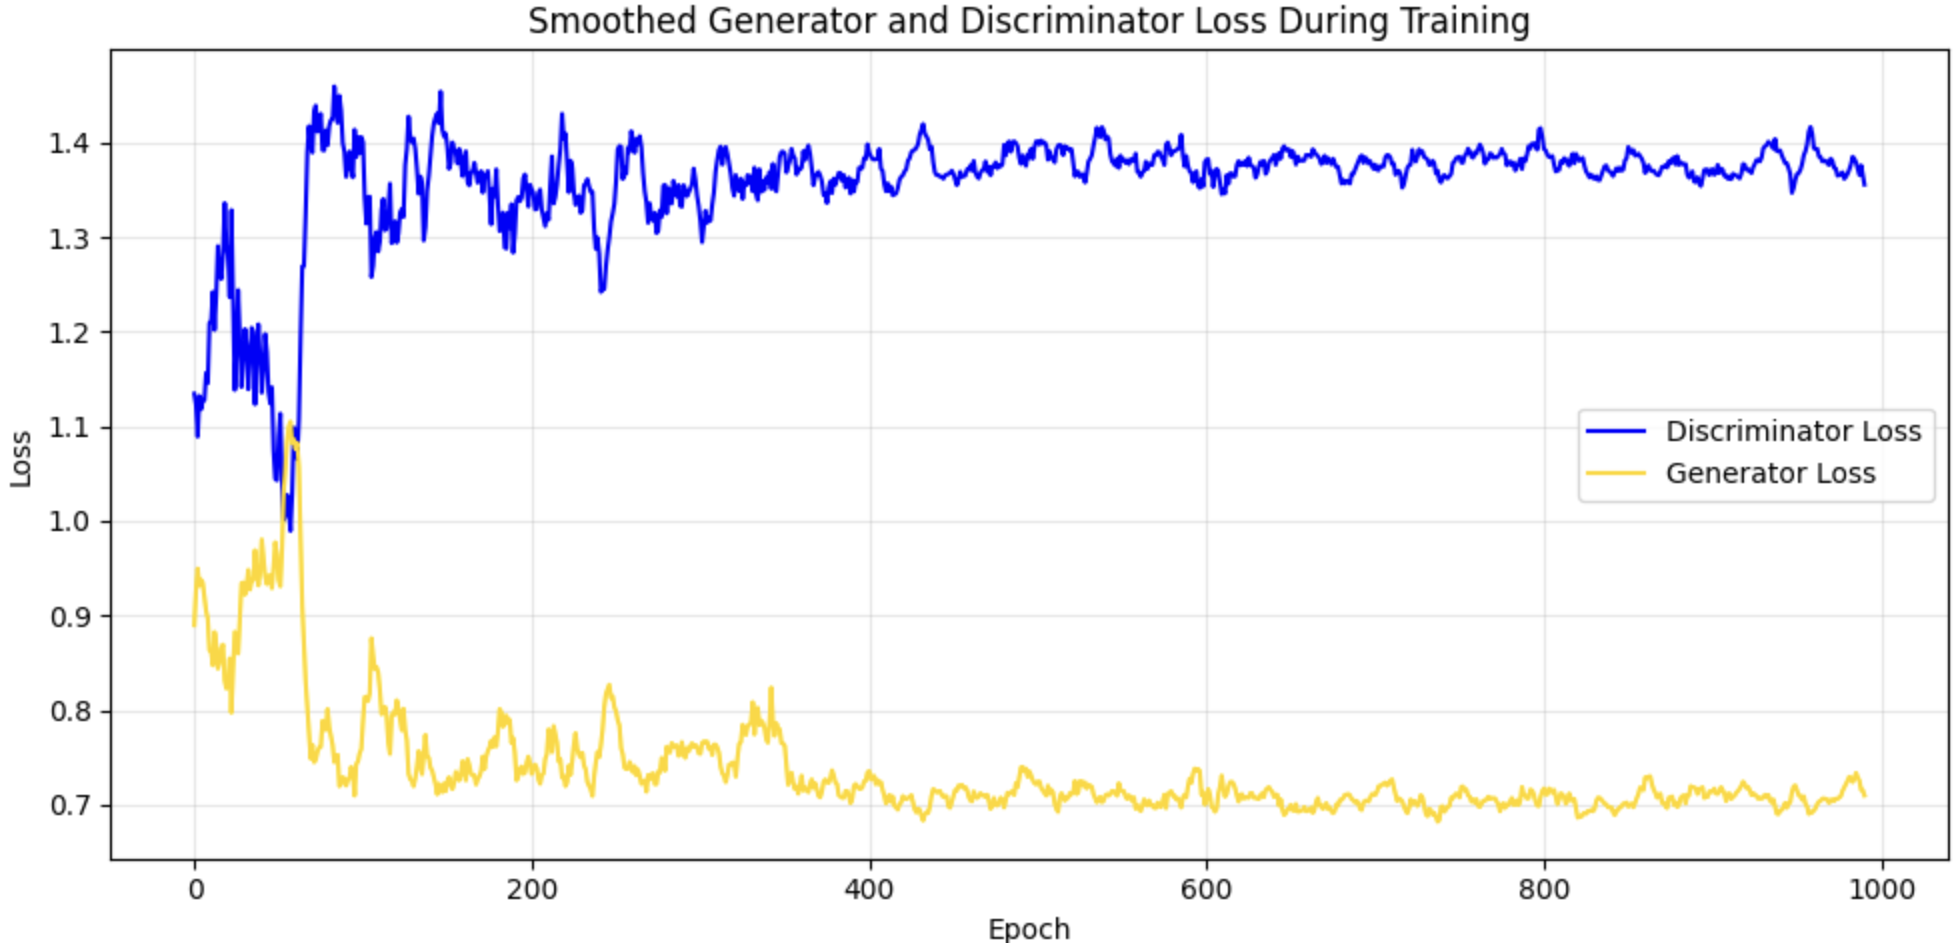
\includegraphics[width=6in]{loss_curve.png}
\caption{Generator and Discriminator loss over epochs.}
\label{fig:loss_curve}
\end{figure*}

Figure~\ref{fig:loss_curve} illustrates how the generator and discriminator losses stabilize as training proceeds. Initially, the discriminator quickly learns to distinguish real from fake data, resulting in a sharp drop in its loss. As the generator improves in mimicking the real data distribution, the discriminator's loss increases, indicating it is becoming harder to differentiate between real and generated data.

We studied the impact of various batch sizes and network capacities. Smaller models exhibited high sensitivity to noise and unstable training dynamics. In contrast, very large models struggled with generalization and showed signs of overfitting and gradient instability.

To address training stability across batch sizes(final batch size is 16) , we adjusted the learning rate—increasing it for larger batch sizes. This adaptation helped counteract vanishing gradients and led to more stable convergence.

Overall, the results reflect the dynamic adversarial relationship between the generator and discriminator, where improvements in one compel adaptive responses from the other, culminating in high-quality synthetic data generation.

Figure~\ref{fig:kde_plot} presents the KDE plot of marginal distributions. It shows a close overlap between the real and synthetic data distributions, suggesting the generator has effectively learned the overall structure of the dataset.

To assess inter-feature dependencies, we generated correlation heatmaps for both real and synthetic data.

\begin{figure*}[!ht]
\centering
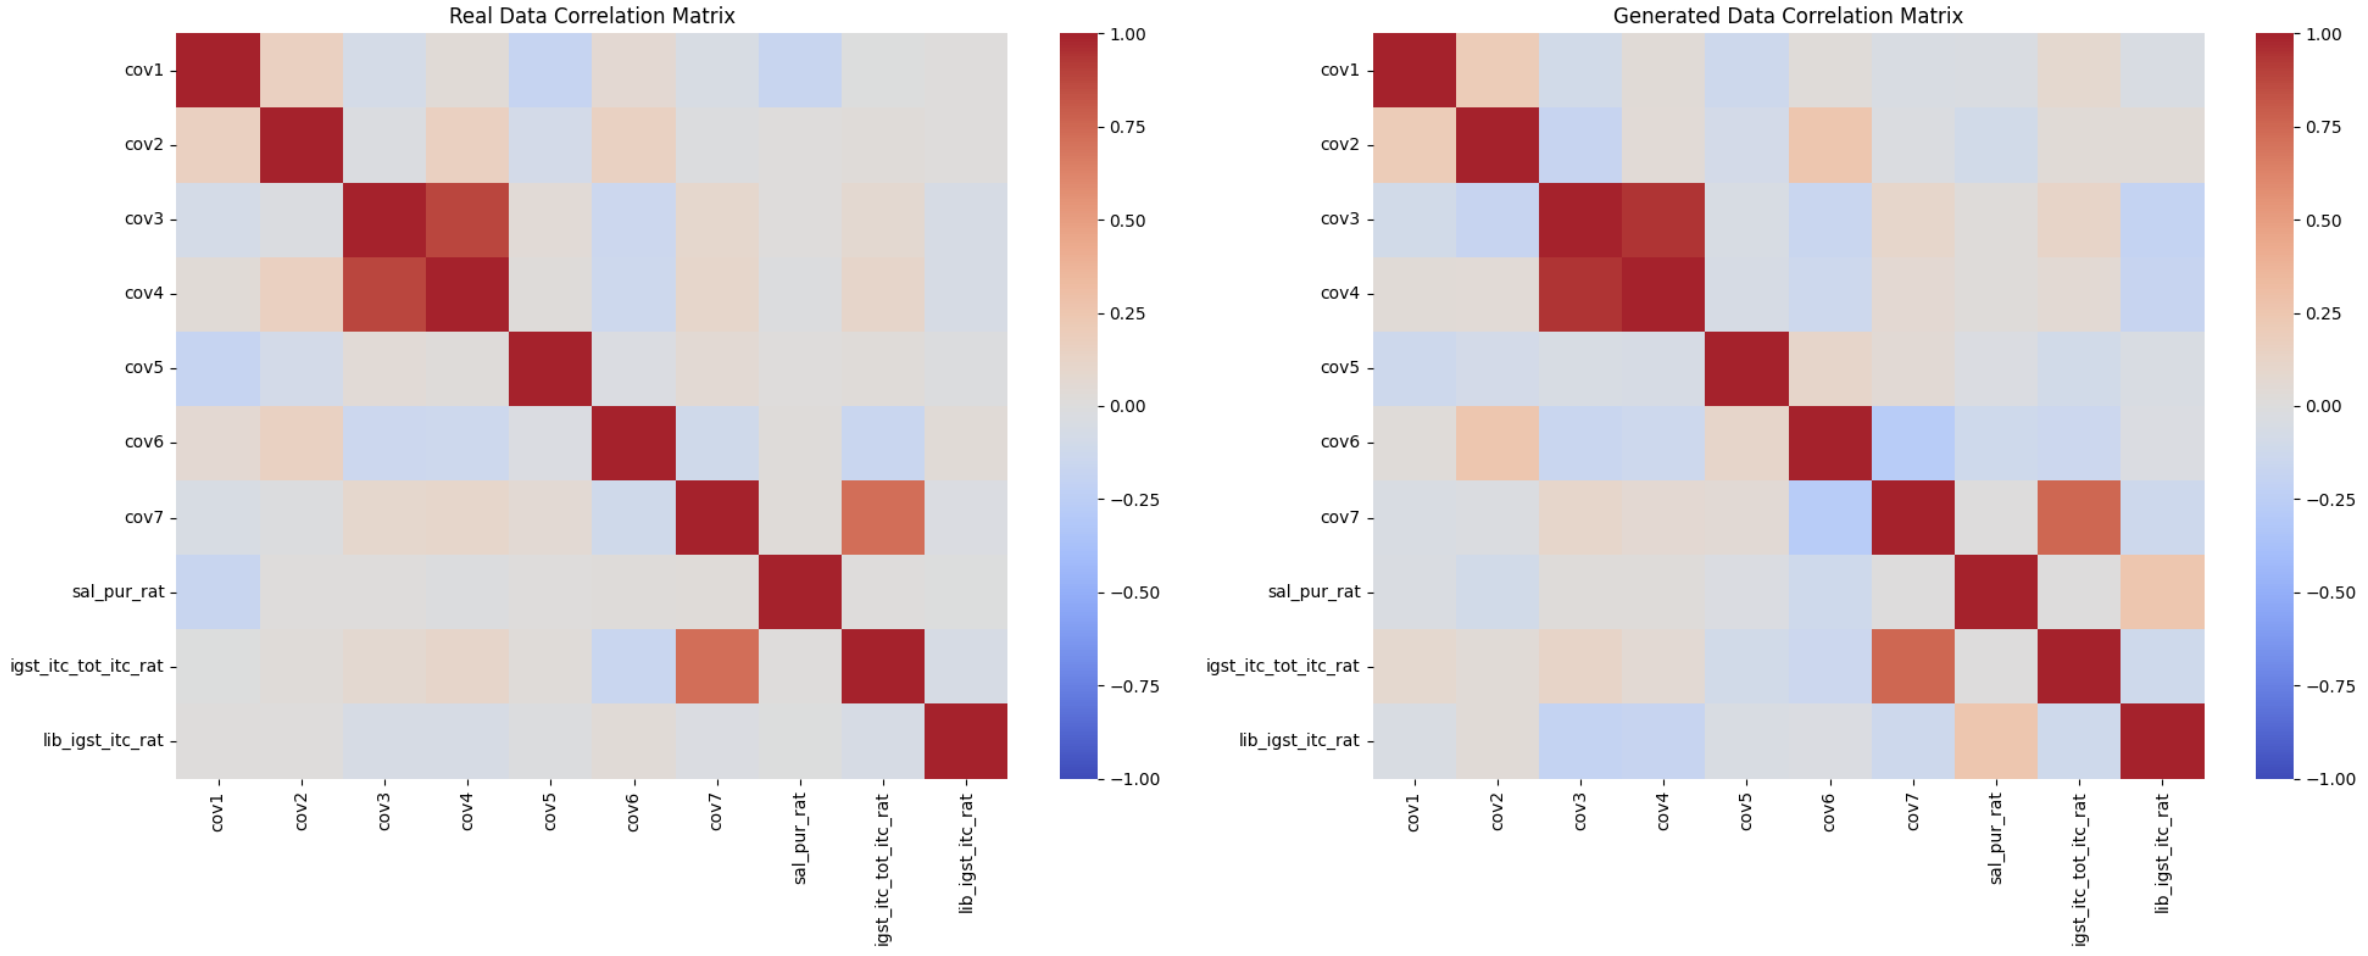
\includegraphics[width=6in]{correlation.png}
\caption{Feature correlation heatmaps for real vs. synthetic data.}
\label{fig:correlation_heatmap}
\end{figure*}

As illustrated in Figure~\ref{fig:correlation_heatmap}, the correlation structure of the synthetic data closely resembles that of the real dataset. This indicates that the model has not only captured marginal distributions but also the relationships among features.

We computed the average absolute differences in pairwise feature correlations, as listed below:

\begin{verbatim}
cov1                    0.044402
cov2                    0.057986
cov3                    0.055450
cov4                    0.050801
cov5                    0.057376
cov6                    0.067205
cov7                    0.038707
sal_pur_rat             0.074341
igst_itc_tot_itc_rat    0.043871
lib_igst_itc_rat        0.084136
\end{verbatim}

These values indicate that the average correlation deviations are low, confirming that the GAN successfully modeled both individual feature distributions and their dependencies.

\begin{figure*}
\centering
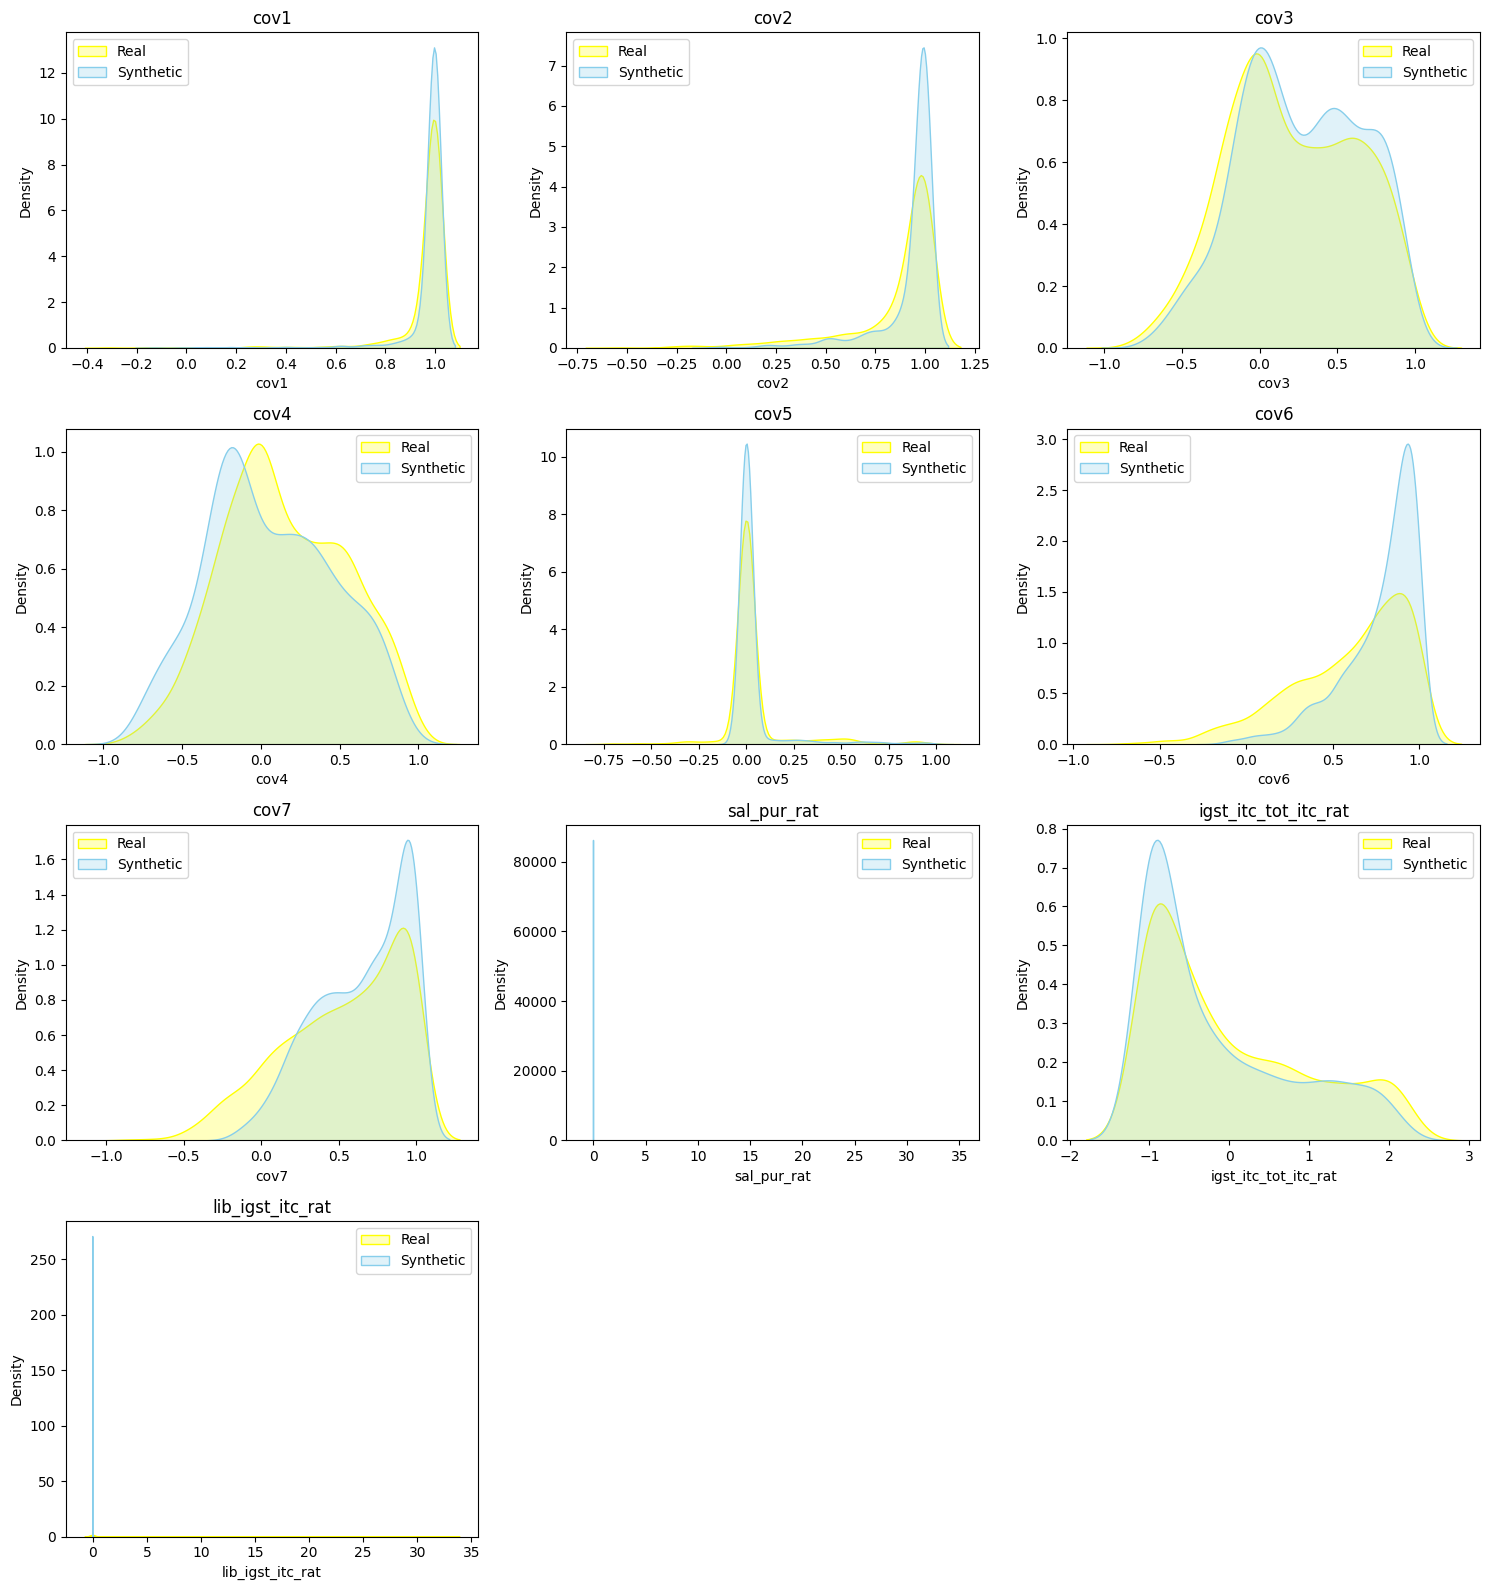
\includegraphics[width=0.9\linewidth]{output.png}
\caption{KDE plot comparing marginal distributions of real and synthetic data.}
\label{fig:kde_plot}
\end{figure*}

\end{document}
